\chapter{Thin Film Growth}
\label{ch:SampFab}
\thispagestyle{empty}


%%%%%%%%%%%%%%%%%%%%%%%%%%%%%%%%%%%%%%%%%%%%%%%%%%%%%%%%%%
%%%%%%%%%%%%%%%%%%%%%%%%%%%%%%%%%%%%%%%%%%%%%%%%%%%%%%%%%%
%%%%%%%%%%%%%%%%%%%%%%%%%%%%%%%%%%%%%%%%%%%%%%%%%%%%%%%%%%

\section{Precursor Selection}
\label{sec:SampFab-Precursors}

\lipsum

%%%%%%%%%%%%%%%
\subsection{Titanium Source}

The source of titanium that was used was titanium(IV) isopropoxide (\TiOiPr{}, \ce{Ti(OCH(CH3)2)4}). This compound is very commonly used in ALD literature.\cite{cianci_atomic_2012,tallarida_growth_2011,lehnert_plasma_2012,cleveland_role_2012,kubrin_stacking_2012,lee_emph-situ_2012} It is a liquid precursor with a high vapor pressure and reacts easily with most oxidizers; the most commonly used oxidant for this reaction is water vapor, similar to the TMA-\ce{H2O} reaction (see Section~\vref{sec:Synth-ALD}). 

%%%%%%%%%%%%%%%
\subsection{Lead Source}

One of the primary tasks of this project was to identify viable ALD precursors for the deposition of lead into the thin films. Potential candidates needed to meet a few stipulations. First, it needed to have chemical and thermal properties compatible with the ALD reactor. It was also desired that previous studies had used it in other ALD processes. Finally, it was important that the compound was available in quantity from chemical suppliers. 

To this end, there were four potential candidates that were investigated which were identified from previous literature reports: tetraphenyllead (\ce{Ph4Pb})\cite{harjuoja_2006}, lead(II) bis(2,2,6,6-tetramethyl-3,5-heptanedionato) (\ce{Pb(TMHD)2})\cite{watanabe_growth_2007}, lead(II) hexafluoroacetylacetonate (\ce{Pb(HFAc)2})\cite{Igumenov_1998}, and lead bis(3-N,N-dimethyl-2-methyl-2- propanoxide) \\\noindent(Pb(DMAMP)$_{2}$).\cite{Hwang_2007}

\ce{Ph4Pb} was one of the commonly used compounds in both ALD and MOCVD references, but it was found to have insufficient volatility for use in the ALD (up to its maximum evaporation temperature of 200\degC{})\cite{harjuoja_2006} and was thus discarded as a candidate. \TMHD{} was another commonly referenced precursor\cite{watanabe_growth_2007}, as was \HFAc{}.\cite{Igumenov_1998} \ce{Pb(DMAMP)2} was seemingly a viable choice, with a very high vapor pressure at low temperatures,\cite{Hwang_2007} but it was not readily available from chemical suppliers and was very costly to purchase which kept it from being considered further. 

Thus, the two compounds \HFAc{} and \TMHD{} were investigated in detail as potential candidates for the lead precursor in the ALD deposition of \PTO{}. Samples of both precursors were obtained from Strem Chemicals, Inc.\cite{strem_inc} and were analyzed to determine which would be most viable. Tests included thermogravimetric analysis (TGA), differential scanning calorimetry (DSC), as well as test depositions of ALD films. 

%%%%%%%%%%%%%%%

\subsection{Oxidizer}

Three potential oxidants were considered; these included water, oxygen, and an ozone/oxygen mix. The choice of oxidant depends heavily on the reactivity with the potential precursors. 

The choice of titanium(IV) isopropoxide as the titanium source allows for any of the three selected oxidizers to be used. A hydrolysis reaction will occur when exposed to water vapor; in the case of oxygen or ozone the ligands will be consumed via a combustion reaction.\cite{ALD-Handbook,Leskela_2002,lim_atomic_2003}

Based on literature reports, the two lead precursors under investigation do not undergo hydrolysis when exposed to water, and as such require the use of the combustion pathway. In addition, through the deposition of test films, it was found that the reaction proceeded more completely when the \ce{O3}/\ce{O2} mixture was used. For simplicity of the process, the \ce{O3}/\ce{O2} mix was used for both half-reactions.\cite{KeunKim2005103}


%%%%%%%%%%%%%%%

\subsection{Proposed Reaction Pathway}

The reaction pathway seen in figure~\vref{fig:PTO-pathway} is a simplified graphical visualization (in the same character as that seen in figure~\vref{fig:TMA-illustration} for TMA) of ALD deposition using \TMHD{} and \TiOiPr{} and an \ce{O2}/\ce{O3} mixture as an oxidant.  

The chemical reactions seen below (in reactions R~\ref{rxn:PTO-Pb1}--\ref{rxn:PTO-Ti2}) also propose a preliminary mechanism for the chemisorption and oxidation/combustion of the precursors to deposit the film. As the materials involved are rather large, in particular \TMHD{}, the molecules have a large stearic hindrance once the chemisorption begins. This impedes the deposition of more than a small fraction of a monolayer per cycle, with lead depositing more slowly than titanium. Therefore, it is likely to have to apply the \TMHD{} half-reaction more often than the \TiOiPr{} reaction when depositing the material. 

{\footnotesize \addtocounter{reaction}{-2} \onehalfspacing
\begin{reactions}
	Pb(TMHD)2 + M-OH_{surf} &-> M-O-Pb(TMHD)_{\,surf} + H(TMHD) \label{rxn:PTO-Pb1}%
%		\AddRxnDesc{PTO: Pb(TMHD) chemisorption}%
		\\
	M-O-Pb(TMHD)_{\,surf} + xO2 + xO3 &-> M-O-Pb(OH)3_{\,surf} + yCO2 + zH2O \label{rxn:PTO-Pb2}%
%		\AddRxnDesc{PTO: Pb(TMHD) oxidation}
		\\
	Ti(OCH(CH3)2)4 + M-OH_{surf} &-> M-O-Ti(OCH(CH3)2)3_{\,surf} + HOC3H7 \label{rxn:PTO-Ti1}%
%		\AddRxnDesc{PTO: Pb(TMHD) chemisorption}%
		\\
	M-O-Ti(OCH(CH3)2)3_{\,surf} + xO2 + xO3 &-> M-O-Ti(OH)3_{\,surf} + yCO2 + zH2O \label{rxn:PTO-Ti2}%
%		\AddRxnDesc{PTO: Pb(TMHD) oxidation}%
\end{reactions}
}

\begin{figure}[tbp]
   \centering
   \subfloat[][Ti Precursor injection]{%
%   	\label{fig:Q50-image}%
	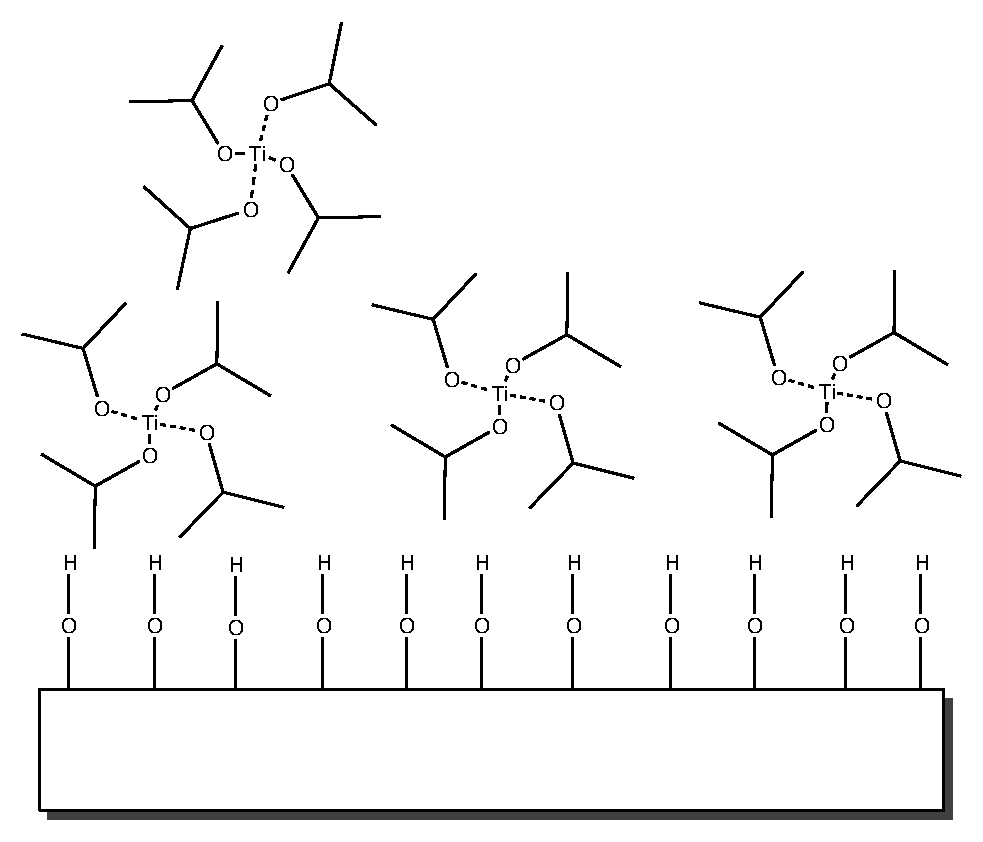
\includegraphics[width=5cm]{./figures/synthesis/chemdraw/a}%
	} 
	\hspace{1cm}
  \subfloat[][Ti Chemisorption]{%
%   	\label{fig:Q50-image}%
	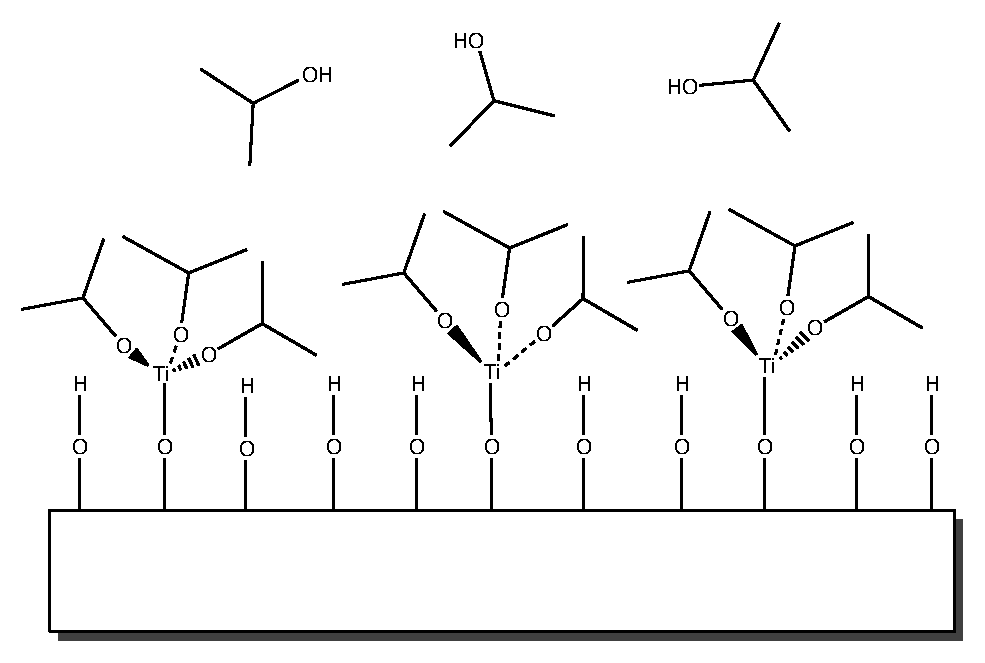
\includegraphics[width=5cm]{./figures/synthesis/chemdraw/b}%
	} \\
  \subfloat[][Ti Ligand Oxidation]{%
%   	\label{fig:Q50-image}%
	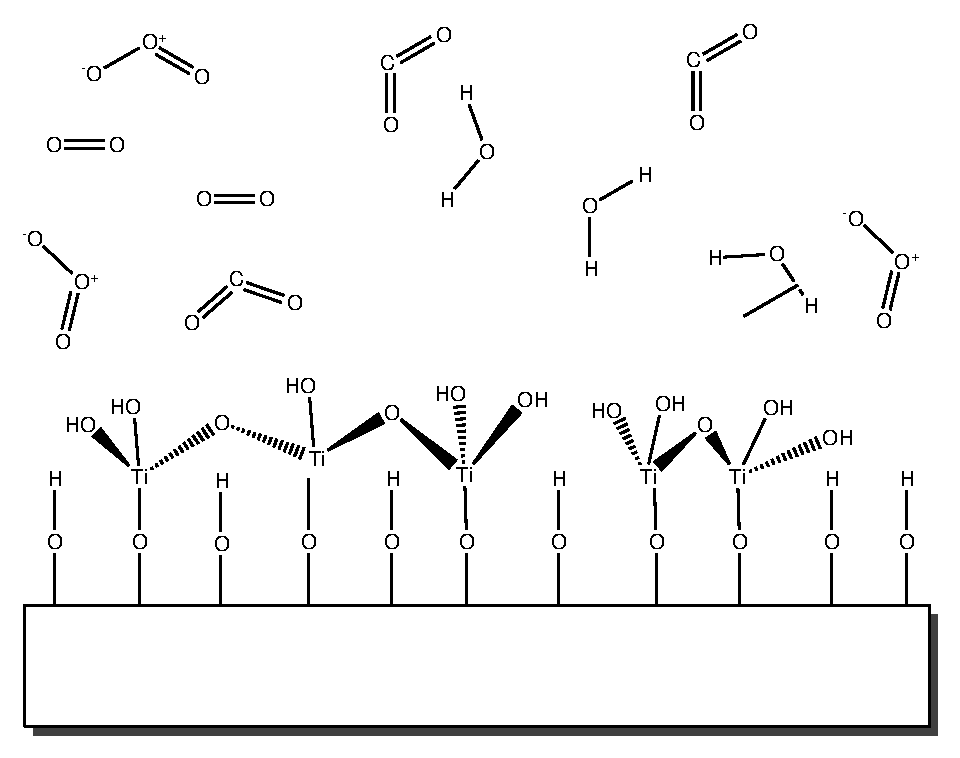
\includegraphics[width=5cm]{./figures/synthesis/chemdraw/c}%
	}  
	\hspace{1cm}	
  \subfloat[][Pb Precursor Injection]{%
%   	\label{fig:Q2000-image}%
	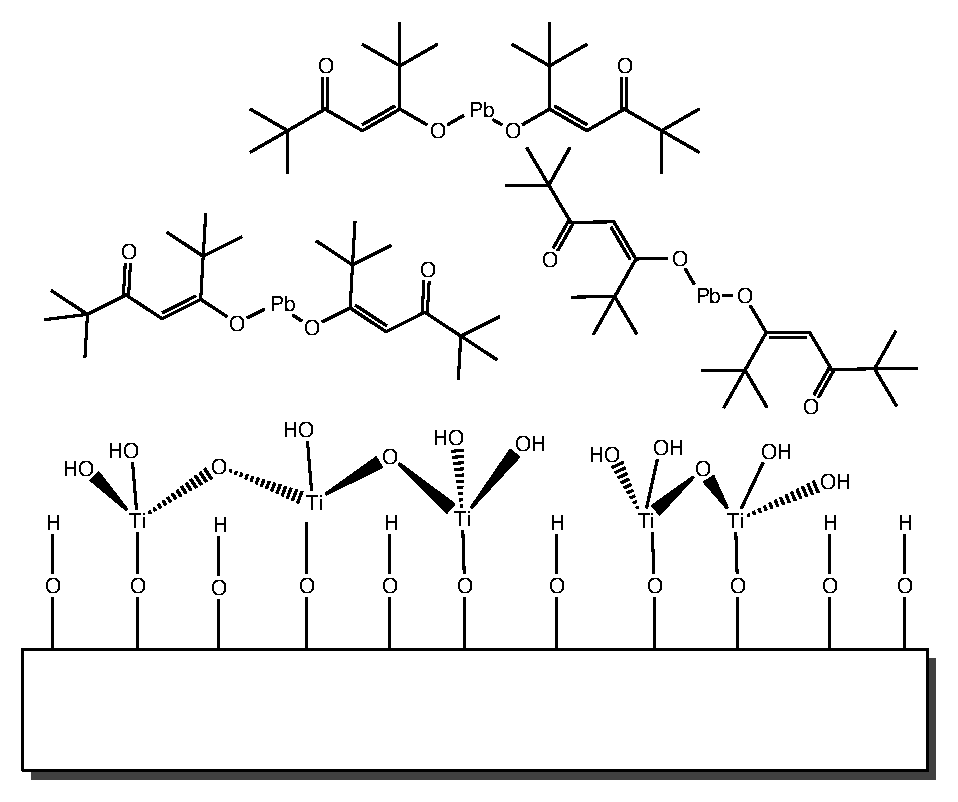
\includegraphics[width=5cm]{./figures/synthesis/chemdraw/d}%
	} \\
  \subfloat[][Pb Chemisorption]{%
%   	\label{fig:Q2000-image}%
	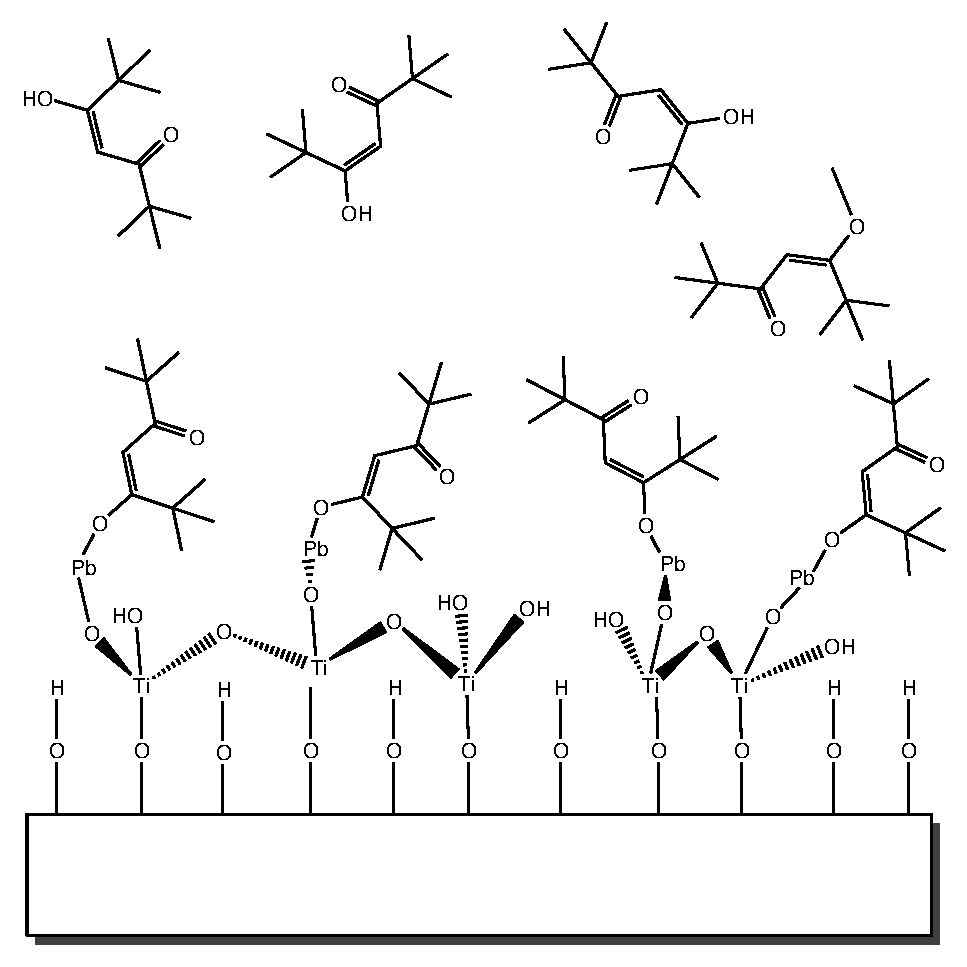
\includegraphics[width=5cm]{./figures/synthesis/chemdraw/e}%
	} 
	\hspace{1cm} 
  \subfloat[][Pb Ligand Oxidation]{%
%   	\label{fig:Q2000-image}%
	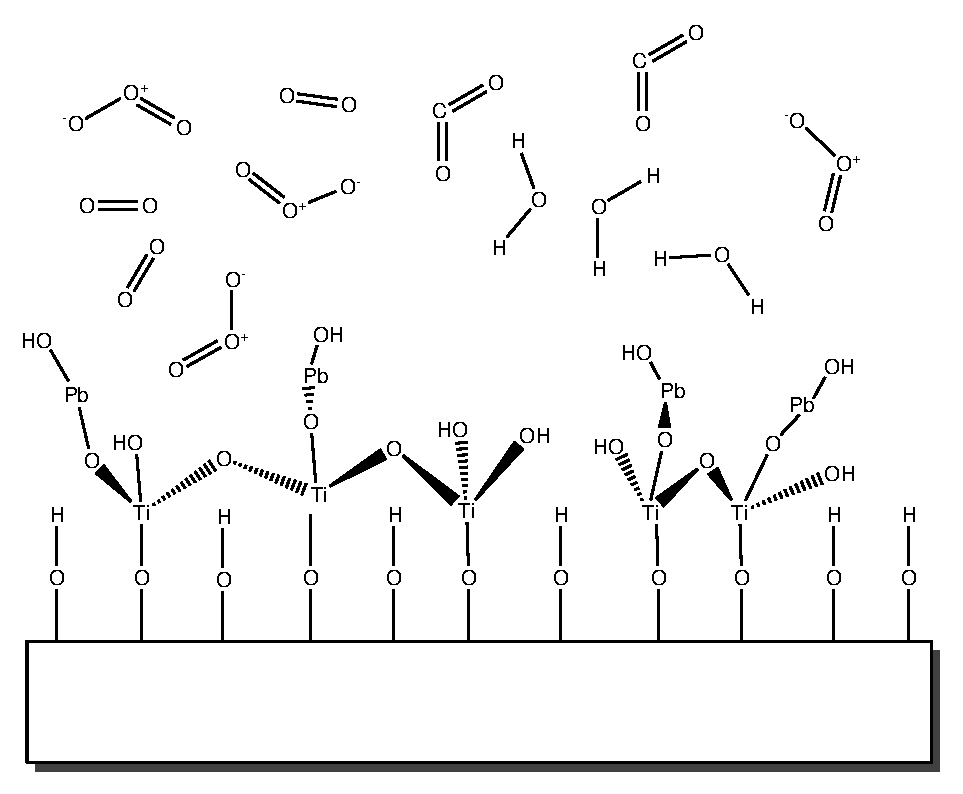
\includegraphics[width=5cm]{./figures/synthesis/chemdraw/f}%
	} \\
  \subfloat[][Completed Cycle, Regenerated Surface]{%
%   	\label{fig:Q2000-image}%
	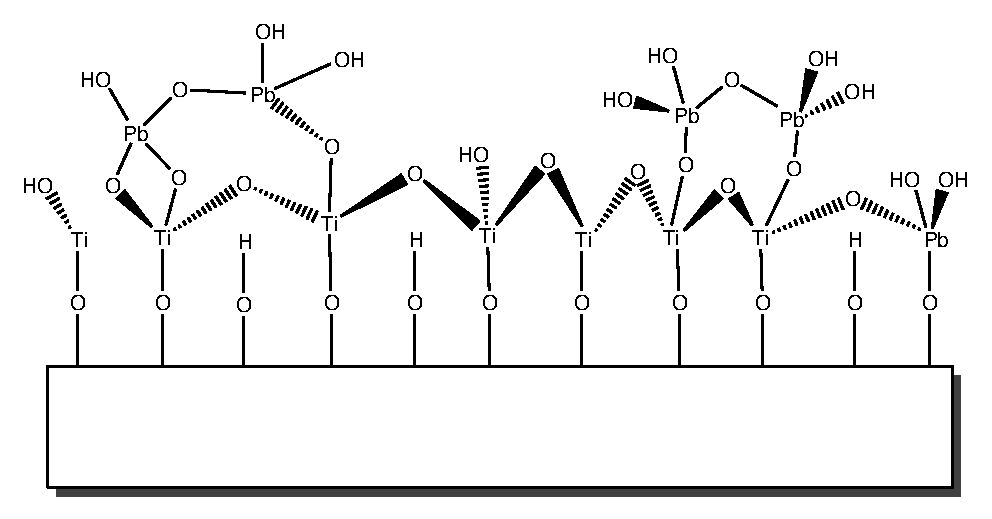
\includegraphics[width=5cm]{./figures/synthesis/chemdraw/g}%
	} 	
   \caption[Illustration of Example \PTO{} ALD Cycle]%
   		{Proposed schematic of \TMHD{} and \TiOiPr{} based ALD deposition for \PTO{}. Purging steps %
		are omitted from this diagram, but would be present between each injection. Steps (d)--(f) would be %
		repeated to incorporate more lead into the film.}
   \label{fig:PTO-pathway}
\end{figure}


%%%%%%%%%%%%%%%%%%%%%%%%%%%%%%%%%%%%%%%%%%%%%%%%%%%%%%%%%%
%%%%%%%%%%%%%%%%%%%%%%%%%%%%%%%%%%%%%%%%%%%%%%%%%%%%%%%%%%
%%%%%%%%%%%%%%%%%%%%%%%%%%%%%%%%%%%%%%%%%%%%%%%%%%%%%%%%%%

\section{Substrate Preparation}
\label{sec:SampFab-Substrates}

Fabrication and preparation of substrates was an important part of the deposition process. Some substrates were purchased and simply cleaned, others needed to be fabricated or otherwise processed prior to cleaning and use in deposition. Three main types of substrates were used: thermally oxidized single-crystalline silicon (100) wafers, silicon wafers that had a thin layer of platinum deposited on the surface, and strontium titanate (100) single crystal substrates. 

%%%%%%%%%%%%%%%
\subsection{Si(100)} \label{sec:Si}

The silicon substrates were prepared in a simple manner. 4 in. diameter silicon wafers with 200 nm of thermally grown oxide (purchased from University Wafer, Inc.\cite{strem_inc}) were diced into 1.5 cm x 1.5 cm pieces. When a sample was to be used for deposition, it was cleaned by one minute of sonication in acetone, followed by isopropanol, with a subsequent 5 minutes of sonication in deionized (DI) water. These were then air dried with dry nitrogen. Finally, the substrates were cleaned in a oxygen plasma cleaning system to remove any remaining organic residues present on the surface.\cite{kern_handbook_1993} 


%%%%%%%%%%%%%%%

\subsection{Platinized Si(100)}

Platinized silicon substrates were prepared in a similar manner to the Si(100) samples. For the initial platinization, a large piece (5 x 5 cm$^{2}$) of pre-cleaned silicon wafer with a thin layer of native oxide, as opposed to the 200 nm of thermally grown oxide, was prepared in the manner described above.\cite{kern_handbook_1993} Then a 15 nm layer of platinum was deposited via ALD.\cite{Ritala_2003_Pt} The substrates were then cleaved into smaller pieces for subsequent use. 

If the samples are stored, it is recommended to again clean the samples in the standard procedure prior to use (see \vref{sec:Si}).

%%%%%%%%%%%%%%%

\subsection{Single Crystal STO(100)}

Single crystal substrates of strontium titanate (\ce{SrTiO3}(100), STO) were purchased from MTI Crystal, Inc.\cite{MTIXtal_inc} as 5 x 5 x 0.5 mm or 10 x 10 x 0.5 mm pieces. These were subsequently processed in such a fashion as to promote the formation of atomically flat terraces. This has the advantage of promoting a uniform surface species across the entire substrate --- the etching process leaves the substrates uniformly titania-terminated.\cite{koster_quasi-ideal_1998}

To achieve the desired surface, the substrates were first pre-cleaned in a four step sonication process. The crystals were cleaned for five minutes in each of acetone, methanol, and isopropyl alcohol. Subsequently, the substrates were sonicated for fifteen minutes in DI water.\cite{koster_quasi-ideal_1998} Next, the substrates were then immersed into a commercially prepared buffered hydrofluoric acid (BHF) solution to etch for 30 seconds, then removed and flushed with copious quantities of DI water to purge any remaining BHF solution.  Once the sample were thoroughly rinsed, they were dried using dry nitrogen. After the etching process, the substrates were annealed at 950\degC{} for one hour.\cite{koster_quasi-ideal_1998} Atomic force microscopy (AFM) was used to confirm the presence of well-defined atomic terraces. 

If the samples are stored, it is recommended to again clean the samples in the standard procedure (see \vref{sec:Si}).

%%%%%%%%%%%%%%%%%%%%%%%%%%%%%%%%%%%%%%%%%%%%%%%%%%%%%%%%%%
%%%%%%%%%%%%%%%%%%%%%%%%%%%%%%%%%%%%%%%%%%%%%%%%%%%%%%%%%%
%%%%%%%%%%%%%%%%%%%%%%%%%%%%%%%%%%%%%%%%%%%%%%%%%%%%%%%%%%

\section{Deposition Parameters}
\label{sec:SampFab-DepParams}

There are four main parameters that can affect the behavior of an ALD deposition.  These are the growth temperature, the dosage of each precursor, the purge time between doses, and any extended precursor-surface exposure time. 

%%%%%%%%%%%%%%%

\subsection{Growth Temperature}

The temperature of the growth chamber has a strong effect on reaction behavior. ALD reactions are sensitive to temperature, and will only proceed properly within a certain range known as the `ALD window.' Outside of this range, the reaction enters one of a number of different regimes; these are determined by comparing the growth rate of the deposition to that of a reaction in the self-limiting saturated ``ALD mode.''\cite{ALD-Handbook,Leskela_2002,lim_atomic_2003,Ritala_ALD_2003} 

If the growth temperature is less than the lower bound of the ALD window, the two regimes are condensation limited and activation energy limited. Condensation limited growth occurs when the substrate temperature is low enough that precursor condenses onto the surface without reacting with the presented sites. This causes higher than expected growth rates, and a lack of self-limiting behavior. If the reaction instead proceeds into the activation energy limited regime, molecules of precursor lack sufficient energy to react with the surface. This is characterized by lower deposition rates.\cite{ALD-Handbook,Leskela_2002} 

Conversely, if the reactor temperature is excessive the reaction again become anomalous. Decomposition limited growth, characterized by excessive deposition, is a result of thermal cracking of the precursor materials. This reaction is not limited to the surface, and accounts for the extra material being deposited. Lower deposition rates indicate that the temperature is sufficient to cause desorption of previously-reacted material from the sample.\cite{ALD-Handbook,Ritala_ALD_2003} 

For an ALD run to be successful, the acceptable temperature window for all of the reactions should overlap in some temperature range. This can become difficult with reactions requiring multiple metal precursors (e.g. \PTO, a combination of \ce{TiO2} and \ce{PbO}), as these can have widely varying ALD windows for their respective reactions. 

%%%%%%%%%%%%%%%

\subsection{Precursor Dosage}

The dosage of precursor or oxidant to the surface is another parameter of critical importance. An ALD reaction requires a minimal amount of precursor to sufficiently saturate the surface, while it is beneficial to minimize any excess precursor as it will be a wasted byproduct (minimizing costs, environmental impact, etc.). 

The vaporization behavior of the precursor can have a dramatic impact on how simple or difficult it is to deliver a saturating dose to the surface. Some materials have readily available precursors with high vapor pressures; titanium isopropoxide and trimethylaluminum (TMA) are both liquids, and tetrakis(dimethylamido)hafnium (\ce{Hf\{N(CH3)2\}4}) is a low-melting temperature solid. These are commonly used precursors for depositing their respective oxides. This vapor pressure becomes an important consideration when choosing a potential compound for use in ALD (as discussed in Section~\vref{sec:SampFab-Precursors}).\cite{ALD-Handbook,kanjolia_design_2008,Leskela_2002,lim_atomic_2003,Ritala_ALD_2003}

Insufficient dosing is apparent in a deposition run by a slower than average growth rate, or also as a non-uniform deposition rate across the sample. However, overdosing is not readily apparent in an ALD-mode deposition. The dose must be lowered to a point where the dose is insufficient, and then increased back to a saturating level. 

Controlling the dose is dependent on injection time (which is the time the valve between the process line and the precursor storage vessel is open), precursor temperature, and the cycle duration (time between precursor injections). By increasing either the injection time or the precursor's temperature the dose is increased, except in some cases with low vapor pressure materials. In this case, it can sometimes be found that the evaporation kinetics are slow and it takes additional time to build up a sufficient amount of vapor to provide a dose to the reactor.\cite{ALD-Handbook,lim_atomic_2003,Ritala_ALD_2003} 

If necessary, multiple doses of precursor can be delivered to the sample during each cycle to increase the total delivered dose.

%%%%%%%%%%%%%%%

\subsection{Purge Time}

Purge time is important as it gives time for the \ce{N2} flow to flush any remaining byproducts, excess reactants, and physisorbed (as opposed to chemisorbed) species from the substrate surface and out of the reactor zone. It also allows time between cycles which allows for low vapor pressure precursors to regenerate evaporated material; if this time is too short to fully regenerate the dose in the cylinder the precursor will eventually appear to be depleted during the course of the deposition.\cite{ALD-Handbook,Leskela_2002}

%%%%%%%%%%%%%%%

\subsection{Exposure Time}

Exposure time denotes the time where the precursor is held in the reaction zone to increase the amount of time during which the surface reaction can occur. This is beneficial for two types of depositions. In the case of low-reactivity precursors, it increases the amount of time that the precursor is available to the surface, greatly increasing the surface coverage per cycle. Exposure mode is also beneficial for depositing upon three dimensional structures, especially those with a high aspect ratio, e.g. nanotube templates. This extra dwell time of the precursor allows for diffusion of reactant into the structure, for a uniform coverage upon the entirety of the surface. Purge time must be increased accordingly to allow for byproducts to diffuse back out of the structure.\cite{ALD-Handbook,gordon_kinetic_2003,Leskela_2002}

%%%%%%%%%%%%%%%%%%%%%%%%%%%%%%%%%%%%%%%%%%%%%%%%%%%%%%%%%%
%%%%%%%%%%%%%%%%%%%%%%%%%%%%%%%%%%%%%%%%%%%%%%%%%%%%%%%%%%
%%%%%%%%%%%%%%%%%%%%%%%%%%%%%%%%%%%%%%%%%%%%%%%%%%%%%%%%%%

\section{Post-Deposition Annealing}
\label{sec:SampFab-Annealing}

Two types of annealing procedures were used in this study. Oven annealing, with the simple use of a furnace in ambient atmosphere; and rapid thermal annealing (RTA), characterized by very high heating and cooling rates and performed in an inert atmosphere (dry \ce{N2}). 


%%%%%%%%%%%%%%%

\subsection{Oven Annealing}

In oven annealing, the samples to be processed are placed in a cold oven in the ambient atmosphere of the laboratory. The samples are then heated gradually at a rate of 10--25\degC{} per minute up to the final annealing temperature, which ranged from 600--900\degC{}. The samples are then allowed to heat-treat for 120 minutes at the process temperature, and then the furnace is allowed to return to room temperature. 

This conventional heating pattern allows the sample to obtain its equilibrium crystalline phase composition, be that a single crystalline phase, polycrystalline, or involve multiple phases or materials. This was the annealing method most commonly used during this study. 

%%%%%%%%%%%%%%%

\subsection{Rapid Thermal Annealing}

Rapid thermal annealing (RTA), as its name suggests, involves very high heating and cooling rates. RTA systems can heat at rates over 10\degC{} per second, allowing the chamber and sample to reach the process temperature very quickly. Similarly, processing times are generally much shorter, and are generally no longer than 10--15 minutes. Cooling, facilitated by a water cooling apparatus, also occurs rapidly. These sharp gradients can have different effects on the crystal structure of the film, locking in different phases in the material that may otherwise dissociate given more time during heating or cooling. 

In this study samples processed via RTA used a HeatPulse\textsuperscript{\texttrademark} RTA system, which allowed for automatic control of the process. Sample processing conditions can be found in table~\vref{tbl:LoSamples}. 





